\documentclass[11pt]{article}
\newif\ifko\kotrue
\newcommand{\shorttitle}{전경 작업 보호형 Windows 자원 조정}
% Shared preamble for the Korean and English RamFlow papers.
% Each main file defines \ifko (true for Korean) before \input-ing this file.
\usepackage[a4paper,top=24mm,bottom=26mm,left=25mm,right=25mm,headsep=8mm,footskip=11mm]{geometry}
\usepackage{amsmath,amssymb}
\usepackage{mathpazo}
\usepackage[no-math]{fontspec}
\ifko
  % Korean: Noto CJK KR carries both Hangul and Latin glyphs, so one family
  % keeps the colour of the page even. Lines break at inter-word spaces.
  \setmainfont{Noto Serif CJK KR}[Scale=0.94,BoldFont={* SemiBold}]
  \setsansfont{Noto Sans CJK KR}[Scale=0.92,BoldFont={* Bold}]
  \setmonofont{DejaVu Sans Mono}[Scale=0.80]
  \linespread{1.30}
  \XeTeXlinebreaklocale "ko"
  \XeTeXlinebreakskip=0pt plus 0.6pt
  \AtBeginDocument{\renewcommand{\emph}[1]{\textsf{#1}}}
  % inside diagrams and tables, break only at spaces and never letter-space
  \AtBeginDocument{\tikzset{every picture/.append style={execute at begin picture={\XeTeXlinebreaklocale ""\XeTeXlinebreakskip=0pt\relax},execute at end picture={\XeTeXlinebreaklocale "ko"}}}}
  \renewcommand{\figurename}{그림}
  \renewcommand{\tablename}{표}
  \renewcommand{\contentsname}{차례}
  \renewcommand{\appendixname}{부록}
  \renewcommand{\abstractname}{초록}
  \AtBeginDocument{\floatname{algorithm}{알고리즘}}
  \AtBeginDocument{\renewcommand{\figurename}{그림}\renewcommand{\tablename}{표}}
\else
  \setmainfont{TeX Gyre Pagella}
  \setsansfont{Noto Sans CJK KR}[Scale=0.92]
  \setmonofont{DejaVu Sans Mono}[Scale=0.80]
  \linespread{1.12}
\fi
\usepackage{microtype}
\setlength{\emergencystretch}{1.5em}
\usepackage{xcolor}
\definecolor{accent}{HTML}{2A78D6}
\definecolor{offc}{HTML}{EB6834}
\definecolor{ink2}{HTML}{52514E}
\definecolor{rule}{HTML}{D9D8D3}
\definecolor{panel}{HTML}{F4F3F0}
\usepackage{graphicx}
\usepackage{booktabs,tabularx,multirow,array}
\usepackage{caption}
\captionsetup{font=small,labelfont={bf,sf},labelsep=period,skip=5pt}
\usepackage{enumitem}
\setlist{itemsep=1pt,topsep=3pt,leftmargin=1.6em}
\usepackage{tikz}
\usetikzlibrary{arrows.meta,positioning,fit,calc,backgrounds,shapes.geometric}
\usepackage{algorithm}
\usepackage[noend]{algpseudocode}
\usepackage{titlesec}
\titleformat{\section}{\large\sffamily\bfseries}{\color{accent}\thesection}{0.8em}{}
\titleformat{\subsection}{\normalsize\sffamily\bfseries}{\color{accent}\thesubsection}{0.7em}{}
\titleformat{\paragraph}[runin]{\normalsize\sffamily\bfseries}{}{}{}[.]
\titlespacing*{\section}{0pt}{14pt plus 3pt}{6pt}
\titlespacing*{\subsection}{0pt}{10pt plus 2pt}{4pt}
\titlespacing*{\paragraph}{0pt}{6pt plus 1pt}{0.6em}
\usepackage{fancyhdr}
\pagestyle{fancy}\fancyhf{}
\renewcommand{\headrulewidth}{0pt}
\fancyhead[L]{\footnotesize\sffamily\color{ink2}RamFlow}
\fancyhead[R]{\footnotesize\sffamily\color{ink2}\shorttitle}
\fancyfoot[C]{\footnotesize\sffamily\color{ink2}\thepage}
\fancypagestyle{plain}{\fancyhf{}\fancyfoot[C]{\footnotesize\sffamily\color{ink2}\thepage}}
\usepackage[hidelinks,unicode]{hyperref}
\hypersetup{colorlinks=true,linkcolor=accent,citecolor=accent,urlcolor=accent}
\usepackage{xurl}
\usepackage[numbers,sort&compress]{natbib}
\setlength{\bibsep}{2pt plus 1pt}
\renewcommand{\bibfont}{\small}
\tikzset{prose/.style={}}
\ifko\tikzset{prose/.style={execute at begin picture={\XeTeXlinebreaklocale "ko"\XeTeXlinebreakskip=0pt plus 0.6pt\relax}}}\fi
\newcommand{\KoEn}[2]{\ifko #1\else #2\fi}
\newcommand{\code}[1]{\texttt{#1}}
\newcommand{\pct}{\%}
% Generated by paper/analysis/analyze.py -- do not edit by hand.
\newcommand{\numCSOff}{88.15}
\newcommand{\numCSOn}{48.14}
\newcommand{\numCSRed}{45.4}
\newcommand{\numCSBlkMed}{41.0}
\newcommand{\numCSBlkMin}{39.2}
\newcommand{\numCSBlkMax}{57.3}
\newcommand{\numCSGmRed}{46.5}
\newcommand{\numCSGmLo}{34.9}
\newcommand{\numCSGmHi}{55.9}
\newcommand{\numCSOffFifty}{76.55}
\newcommand{\numCSOnFifty}{38.73}
\newcommand{\numCOOff}{88.56}
\newcommand{\numCOOn}{48.95}
\newcommand{\numCORed}{44.7}
\newcommand{\numCOBlkMed}{39.6}
\newcommand{\numCOBlkMin}{37.2}
\newcommand{\numCOBlkMax}{53.2}
\newcommand{\numCOGmRed}{43.3}
\newcommand{\numCOGmLo}{33.6}
\newcommand{\numCOGmHi}{51.5}
\newcommand{\numCOOffFifty}{76.44}
\newcommand{\numCOOnFifty}{39.35}
\newcommand{\numVCOff}{99.36}
\newcommand{\numVCOn}{50.52}
\newcommand{\numVCRed}{49.2}
\newcommand{\numVCBlkMed}{45.4}
\newcommand{\numVCBlkMin}{43.7}
\newcommand{\numVCBlkMax}{58.1}
\newcommand{\numVCGmRed}{50.5}
\newcommand{\numVCGmLo}{40.4}
\newcommand{\numVCGmHi}{58.9}
\newcommand{\numVCOffFifty}{65.14}
\newcommand{\numVCOnFifty}{38.80}
\newcommand{\numVSOff}{62.46}
\newcommand{\numVSOn}{31.60}
\newcommand{\numVSRed}{49.4}
\newcommand{\numVSBlkMed}{35.8}
\newcommand{\numVSBlkMin}{26.3}
\newcommand{\numVSBlkMax}{63.7}
\newcommand{\numVSGmRed}{43.4}
\newcommand{\numVSGmLo}{19.1}
\newcommand{\numVSGmHi}{60.4}
\newcommand{\numVSOffFifty}{34.97}
\newcommand{\numVSOnFifty}{23.50}
\newcommand{\numBgCOff}{267,405}
\newcommand{\numBgCOn}{107,056}
\newcommand{\numBgCRed}{60.0}
\newcommand{\numBgVOff}{220,064}
\newcommand{\numBgVOn}{87,371}
\newcommand{\numBgVRed}{60.3}
\newcommand{\numEfSOff}{72.70}
\newcommand{\numEfSOn}{44.40}
\newcommand{\numEfOOff}{83.00}
\newcommand{\numEfOOn}{46.90}
\newcommand{\numSessions}{10}
\newcommand{\numSessionsOk}{10}
\newcommand{\numPooledP}{0.0020}
\newcommand{\numTasks}{1,200}
\newcommand{\numConditions}{20}
\newcommand{\numMxOff}{232.85}
\newcommand{\numMxOn}{131.32}
\newcommand{\numMxRed}{43.6}
\newcommand{\numMxBlkMin}{39.7}
\newcommand{\numMxBlkMax}{43.8}
\newcommand{\numMxGmLo}{40.3}
\newcommand{\numMxGmHi}{44.6}
\newcommand{\numMxOffFifty}{223.60}
\newcommand{\numMxOnFifty}{129.01}
\newcommand{\numMxFiftyRed}{42.3}
\newcommand{\numMxBgRed}{59.6}
\newcommand{\numMxAvLo}{856.8}
\newcommand{\numMxAvHi}{1144.0}
\newcommand{\numCpOff}{230.78}
\newcommand{\numCpOn}{219.76}
\newcommand{\numCpRed}{4.8}
\newcommand{\numCpBlkMin}{0.9}
\newcommand{\numCpBlkMax}{6.0}
\newcommand{\numCpGmLo}{1.8}
\newcommand{\numCpGmHi}{6.6}
\newcommand{\numCpOffFifty}{227.62}
\newcommand{\numCpOnFifty}{128.99}
\newcommand{\numCpFiftyRed}{43.3}
\newcommand{\numCpBgRed}{38.4}
\newcommand{\numCpAvLo}{14425.9}
\newcommand{\numCpAvHi}{15157.5}
\newcommand{\numScAmb}{1,811.26}
\newcommand{\numScAbs}{1,896.05}
\newcommand{\numScDry}{1,853.10}
\newcommand{\numScLive}{1,877.65}
\newcommand{\numScDiff}{−18.40}
\newcommand{\numScDiffPct}{−0.97}
\newcommand{\numCiLevel}{93.8}
\newcommand{\numSignP}{0.0312}
\newcommand{\numWilP}{0.0625}

% A rounded "finding" box used for key takeaways
\newcommand{\finding}[1]{%
  \par\smallskip\noindent
  \begin{tikzpicture}[prose]
    \node[fill=panel,rounded corners=3pt,inner sep=7pt,text width=\dimexpr\linewidth-14pt\relax,align=left]{\small #1};
    \fill[accent,rounded corners=1pt] ($(current bounding box.north west)+(0,-1pt)$) rectangle ($(current bounding box.south west)+(2.2pt,1pt)$);
  \end{tikzpicture}\par\smallskip}

\graphicspath{{../figures/}}

\begin{document}
\thispagestyle{plain}

\begin{center}
{\sffamily\bfseries\LARGE RamFlow\par}
\vspace{4pt}
{\sffamily\large 메모리를 비우는 대신 현재 작업을 지키는\\보수적·가역적 Windows 자원 조정: 설계와 단일 PC 실측 연구\par}
\vspace{10pt}
{\normalsize homesweetlove\par}
{\small\color{ink2}\url{https://github.com/homesweetlove/RamFlow_Windows}\par}
\vspace{2pt}
{\small\color{ink2}기술 보고서 · 2026년 11월 · 영어판: \texttt{paper/en/RamFlow-paper-en.pdf}\par}
\end{center}

\vspace{4pt}
\noindent\begin{tikzpicture}[prose]
\node[fill=panel,rounded corners=4pt,inner sep=10pt,text width=\dimexpr\linewidth-20pt\relax,align=justify]{%
{\sffamily\bfseries 초록}\quad
메모리가 부족한 PC에서 흔히 쓰이는 ``RAM 최적화'' 프로그램은 다른 프로세스의 Working Set(물리 메모리에 올라와 있는 페이지 집합)을 강제로 비워 ``사용 가능한 메모리'' 숫자를 키운다. 그러나 숫자가 커지는 것과 사용자가 지금 쓰는 앱이 빨라지는 것은 다른 문제이다. 본 논문은 Windows용 자원 조정 도구 RamFlow를 설계하고, 다음 질문을 실측으로 확인한다. \emph{메모리를 비우는 대신, 현재 사용 중인 작업을 보호하면서 정해진 배경 작업에만 되돌릴 수 있는 방식으로 양보를 요구하면 전경 응답이 좋아지는가?} RamFlow는 문서화된 공개 API만 사용하고, 사용자 세션의 분리 엔진에서 압박을 추정(EMA·히스테리시스)한 뒤, 보호 규칙을 통과한 프로세스에만 메모리·CPU 우선순위와 EcoQoS를 낮추며, 바꾸기 전에 원래 값을 저널에 기록해 복원한다. 되돌릴 수 없는 Working Set 축소는 가용 물리 RAM이 1\,GiB 미만일 때만 허용한다.
단일 PC(i5-13400, RAM 약 24\,GiB)에서 세 개의 짝지은 실험을 수행했다. (1) Working Set 축소 위주의 정책은 저메모리 전경 작업의 완료 시간을 의미 있게 줄이지 못했고(중앙값 차이 \numScDiffPct\%), 여유 RAM이 있을 때의 축소는 배경 앱의 복귀를 오히려 느리게 했다. (2) 명시적 배경 작업 양보로 바꾼 뒤, 메모리·CPU 경쟁 부하에서 전경 요청의 블록별 p95 지연 중앙값이 \numMxOff\,ms에서 \numMxOn\,ms로 \numMxRed\% 줄었다(5/5 블록 개선). (3) 실제 Chrome과 VS Code에서 검색·정렬·코드 완성·저장 지연이 각각 \numCSRed--\numVSRed\% 줄었고, 앱 세션 \numSessions{}개 모두에서 네 기능이 개선되었다(부호검정 $p=\numPooledP$). 대가로 배경 작업 처리량은 약 60\% 감소했다. 실험 \numTasks{}건의 결과 정확성, 자원 설정 원복, 대상 밖 변경 0건을 확인했다. 결과는 전경 응답성과 배경 처리량의 교환 관계를 보여주며, RAM 단독 효과나 모든 PC에서의 성능 향상을 뜻하지 않는다. 원시 요약 자료와 분석 코드를 함께 공개한다.
\par\smallskip
{\sffamily\bfseries\small 핵심어}\quad{\small 메모리 압박, 전경 응답성, 꼬리 지연, 프로세스 우선순위, EcoQoS, Working Set, 재현 가능한 측정}};
\end{tikzpicture}

%=====================================================================
\section{서론}
\label{sec:intro}

메모리가 넉넉하지 않은 PC에서 브라우저, 편집기, 빌드, 내려받기, 로컬 AI 모델을 함께 돌리면 사용자가 지금 보고 있는 앱이 버벅인다. 이 문제를 해결한다고 내세우는 프로그램은 오래전부터 있었다. 대표적인 것이 ``RAM 최적화'' 또는 ``메모리 부스터''로, 대개 다른 프로세스의 Working Set을 강제로 줄여 작업 관리자의 사용 가능 메모리 숫자를 올린다. Russinovich는 이런 도구가 잘해야 효과가 없고, 나쁘면 성능을 크게 떨어뜨린다고 분석했다\citep{russinovich2004}. 쫓겨난 페이지를 앱이 다시 쓰려면 다시 읽어 와야 하기 때문이다\citep{mswset,denning1968}.

운영체제는 이미 더 정교한 수단을 갖고 있다. macOS는 2013년부터 쓰지 않는 메모리를 압축하고 보이지 않는 앱을 재우며(App Nap)\citep{mavericks2013}, Windows 10은 메모리 압축 저장소를 도입했다\citep{win10compression}. Windows는 배경 작업의 전력 상태를 낮추는 Power Throttling과 EcoQoS를 제공한다\citep{powerthrottling2017,ecoqos2021}. 데이터센터에서는 리눅스 PSI로 ``자원 부족 때문에 잃은 시간''을 직접 재고, 그 신호로 메모리 회수량을 조절한다\citep{psi,weiner2022tmo}.

이 논문은 개인 PC 수준에서 다음 질문을 다룬다. \textbf{가장 많은 RAM을 확보하는 대신, 지금 사용 중인 작업을 보호하면서 사용자가 지정한 배경 작업에만 되돌릴 수 있는 양보를 요구하면, 전경 응답 지연이 실제로 줄어드는가? 그리고 그 대가는 얼마인가?}

이를 위해 Windows용 자원 조정 도구 RamFlow를 만들고, 개발 과정에서 세 번의 실측을 거쳐 설계를 고쳤다. 첫 실험에서 Working Set 축소 위주의 정책이 효과를 보이지 못하자 축소 조건을 강화하고, 배경 작업의 양보를 명시적으로 제어하는 방향으로 바꾸었다. 그 뒤 같은 부하에서 실제 Chrome과 VS Code로 효과가 옮겨 가는지 확인했다. 이 논문의 기여는 다음과 같다.

\begin{enumerate}
  \item \textbf{보수적·가역적 설계.} 문서화된 API만 사용하고, 보호 규칙·히스테리시스·쿨다운·원래 값 저널로 ``틀렸을 때의 피해''를 제한하는 사용자 공간 자원 조정 구조를 제시한다(\S\ref{sec:design}).
  \item \textbf{부정적 결과의 기록.} Working Set 축소가 사용 가능 메모리 숫자를 키워도 전경 성능 이득으로 이어지지 않았고, 여유가 있을 때는 복귀 지연을 키웠다는 실측을 보고하고, 이를 근거로 한 1\,GiB 보호 규칙을 설명한다(\S\ref{sec:rq1}).
  \item \textbf{효과와 비용의 동시 측정.} 명시적 배경 양보가 통제 부하와 실제 앱 모두에서 p95 지연을 약 44--49\% 줄이는 동시에 배경 처리량을 약 60\% 줄인다는 교환 관계를 짝지은 블록 설계로 측정한다(\S\ref{sec:rq2}--\S\ref{sec:rq4}).
  \item \textbf{재현 가능한 공개 자료.} 조건별 요약 CSV, 프로토콜 JSON, 이 논문의 모든 수치와 그림을 다시 만드는 분석 코드를 저장소에 함께 공개한다(부록~\ref{app:repro}).
\end{enumerate}

%=====================================================================
\section{배경과 관련 연구}
\label{sec:background}

\paragraph{Windows 메모리 용어}
\emph{Working Set}은 프로세스가 현재 물리 메모리에 두고 있는 페이지 집합이다\citep{mswset}. Working Set에서 빠진 페이지는 곧바로 사라지지 않고 Standby·Modified 목록에 잠시 남을 수 있으며, 수정된 페이지를 재사용하려면 보조 저장소에 먼저 써야 할 수 있다\citep{mswset}. \emph{Commit}은 시스템이 지급을 약속한 가상 메모리의 총량으로, 물리 RAM과 페이지 파일을 합한 한도(Commit Limit)를 넘을 수 없다. 따라서 Working Set을 줄여도 Commit은 줄지 않는다. 이 차이는 \S\ref{sec:design}의 축소 조건에 그대로 반영된다.

\paragraph{RAM 최적화기 비판}
RAM 최적화기는 사용 가능 메모리 숫자를 올리지만, 그 과정에서 다른 프로세스의 코드와 데이터를 밀어내 나중에 다시 읽게 만든다\citep{russinovich2004}. 1990년대 SoftRAM처럼 ``메모리를 두 배로 늘린다''고 광고했지만 실제로는 거의 아무것도 하지 않은 사례도 분석된 바 있다\citep{chen2021softram}. RamFlow의 첫 실험(\S\ref{sec:rq1})은 이 비판을 현대 Windows 11에서 다시 확인한 셈이다.

\paragraph{운영체제 내장 기법}
macOS의 압축 메모리와 App Nap\citep{mavericks2013}, Windows의 메모리 압축\citep{win10compression}과 Power Throttling\citep{powerthrottling2017}은 커널 안에서 전체 시스템 정보를 갖고 동작한다. EcoQoS는 응용 프로그램이 \code{SetProcessInformation}으로 자기 프로세스나 스레드를 효율 우선으로 표시하는 API이다\citep{ecoqos2021,mssetprocinfo}. RamFlow는 이 공개 API를 \emph{다른} 프로세스에 적용하되, 사용자가 지정했거나 오래 쉬고 있는 프로세스로 한정한다.

\paragraph{압박 신호와 회수 제어}
리눅스 PSI는 CPU·메모리·I/O 부족으로 작업이 멈춘 시간의 비율을 직접 보고한다\citep{psi}. Meta의 TMO는 PSI를 신호로 사용자 공간 에이전트(Senpai)가 컨테이너별 메모리 회수량을 조절해, 대규모 서버군에서 메모리를 20--32\% 절약했다\citep{weiner2022tmo}. 안드로이드의 lmkd는 메모리 압박 시 우선순위가 낮은 앱을 종료한다\citep{lmkd}. Windows에는 PSI와 같은 ``멈춘 시간'' 지표가 공개되어 있지 않아, RamFlow는 가용 RAM·Commit·페이지 입력·Standby 등 대리 지표를 합친 휴리스틱 점수를 쓴다(\S\ref{sec:pressure}). 이 점이 가장 큰 설계상 한계이다.

\paragraph{가장 가까운 선행 도구}
상용 도구 Process Lasso의 ProBalance는 CPU를 독점하는 배경 프로세스의 우선순위 클래스를 일시적으로 Below Normal로 낮추고, 조건이 사라지면 원래대로 되돌려 응답성을 유지한다\citep{probalance}. 배경 프로세스의 우선순위를 낮춰 전경을 지킨다는 핵심 생각은 RamFlow와 같다. RamFlow가 다른 점은 (i) CPU 우선순위뿐 아니라 메모리 우선순위와 EcoQoS를 함께 조정하고, (ii) 메모리 압박 조건과 메모리 여유 기반 작업 큐를 두며, (iii) 바꾸기 전 원래 값과 프로세스 신원을 디스크 저널에 남겨 강제 종료 뒤에도 복원을 재시도하고, (iv) 부정적 결과를 포함한 실측 자료와 분석 코드를 공개한다는 점이다. 우리는 ProBalance와 직접 비교 실험을 하지 않았으므로 두 도구의 우열을 주장하지 않는다.

%=====================================================================
\section{설계 목표와 제약}
\label{sec:goals}

\begin{description}[leftmargin=2.2em,style=nextline,itemsep=2pt]
  \item[G1. 전경 우선] 사용자가 지금 쓰는 앱과, 같은 실행 파일 이름을 가진 관련 프로세스는 어떤 조치의 대상도 되지 않는다.
  \item[G2. 불확실하면 행동하지 않음] 활동 정보를 읽지 못하거나, 전경 창을 확인하지 못하거나, 전체화면이면 새 조치를 하지 않는다.
  \item[G3. 가역성] 되돌릴 수 있는 설정은 바꾸기 \emph{전에} 원래 값을 기록하고, 프로세스 신원(PID와 생성 시각)이 같을 때만 복원한다.
  \item[G4. 되돌릴 수 없는 조치의 최소화] Working Set 축소는 가장 엄격한 조건에서만, 한 번에 한 프로세스만 수행한다.
  \item[G5. 자기 비용 포함] 도구 자신의 메모리와 상주 비용도 측정 대상이다.
\end{description}

\noindent 금지한 수단도 명시한다. 커널 드라이버, 문서화되지 않은 API나 후킹, 프로세스 자동 종료, Realtime 우선순위, Standby 목록 일괄 비우기는 사용하지 않는다. 클라우드 저장소를 RAM이나 페이지 파일처럼 쓰지 않는다.

%=====================================================================
\section{시스템 설계}
\label{sec:design}

\begin{figure}[t]
  \centering
  % System architecture of RamFlow 0.3.4 (+ background-control revision)
\begin{tikzpicture}[
  font=\footnotesize\sffamily\linespread{1.0}\selectfont,
  box/.style={draw=ink2!60,rounded corners=2.5pt,fill=white,align=center,inner sep=4pt,minimum height=9mm,line width=0.5pt,text width=#1},
  box/.default=27mm,
  core/.style={box=#1,fill=accent!7,draw=accent!70},
  core/.default=34mm,
  zone/.style={draw=rule,rounded corners=4pt,fill=panel,inner sep=6pt,line width=0.5pt},
  lab/.style={font=\scriptsize\sffamily\bfseries,text=ink2,anchor=south west,inner sep=2pt},
  note/.style={font=\scriptsize\sffamily,text=ink2,align=center},
  arr/.style={-{Stealth[length=4pt]},ink2,line width=0.55pt},
  darr/.style={{Stealth[length=4pt]}-{Stealth[length=4pt]},ink2,line width=0.55pt}]
  % engine (two columns)
  \node[core] (sense) at (0,0) {\KoEn{자원 센서}{Resource sensors}\\{\scriptsize RAM · Commit · Standby\\Page-in · CPU}};
  \node[core,below=4mm of sense] (press) {\KoEn{압박 추정}{Pressure estimator}\\{\scriptsize EMA $+$ \KoEn{히스테리시스}{hysteresis}}};
  \node[core,below=4mm of press] (prot) {\KoEn{보호 규칙}{Protection rules}\\{\scriptsize \KoEn{전경 · 시스템 · 활성 · 불확실}{foreground, system, active, unknown}}};
  \node[core,right=7mm of sense] (queue) {\KoEn{배경 작업 큐}{Background job queue}\\{\scriptsize \KoEn{메모리 여유 기반 입장}{headroom-based admission}}};
  \node[core,below=4mm of queue] (act) {\KoEn{개입 사다리}{Intervention ladder}\\{\scriptsize \KoEn{메모리·CPU 우선순위 · EcoQoS\\CPU Sets · 조건부 WS 축소}{memory/CPU priority, EcoQoS,\\CPU Sets, gated WS trim}}};
  \node[core,below=4mm of act] (journal) {\KoEn{복원 저널}{Restore journal}\\{\scriptsize \KoEn{원래 값 · PID 신원}{original values, PID identity}}};
  \draw[arr] (sense) -- (press);
  \draw[arr] (press) -- (prot);
  \draw[arr] (press) -- (act);
  \draw[arr] (prot.east) -- ++(3.5mm,0) |- ($(act.west)+(0,-2.5mm)$);
  \draw[arr] (sense) -- (queue);
  \draw[arr] (act) -- (journal);
  \begin{scope}[on background layer]
    \node[zone,fit=(sense)(prot)(queue)(journal)] (eng) {};
  \end{scope}
  \node[lab] at (eng.north west) {\KoEn{분리 엔진 \texttt{RamFlow.Service --serve} · 사용자 세션}{Separate engine \texttt{RamFlow.Service --serve} (user session)}};
  % user-facing processes
  \node[box,left=25mm of sense.west,anchor=east] (ui) {\KoEn{설정·도구 화면}{Settings \& tools UI}\\{\scriptsize WPF}};
  \node[box,below=13mm of ui] (tray) {\KoEn{경량 트레이}{Lightweight tray}\\{\scriptsize WinForms}};
  \draw[darr] (ui) -- node[note,right,xshift=1pt]{\KoEn{준비 확인 후\\WPF 종료}{handoff, then\\WPF exits}} (tray);
  \draw[darr] (ui.east) -- node[note,above]{Named Pipe} node[note,below]{\KoEn{사용자 SID별}{per user SID}} (ui.east -| eng.west);
  \draw[darr] (tray.east) -- (tray.east -| eng.west);
  % OS and service
  \node[box=27mm,draw=ink2!40,text=ink2,below=7mm of tray] (scm) {\KoEn{선택적 SCM 서비스}{Optional SCM service}\\{\scriptsize \KoEn{Session 0 · 관측만}{Session 0, observe only}}};
  \path let \p1=(scm.west), \p2=(eng.east) in node[box=\x2-\x1-8pt,fill=panel,draw=rule,anchor=north west,minimum height=8mm] (os) at ($(scm.south west)+(0,-4mm)$) {\KoEn{문서화된 Windows API만 사용}{Documented Windows APIs only}\\{\scriptsize\texttt{SetProcessInformation} · \texttt{SetPriorityClass} · CPU Sets · PDH · \texttt{EmptyWorkingSet}}};
  \draw[arr] (eng.south) -- (eng.south |- os.north);
  \draw[arr] (scm.south) -- (scm.south |- os.north);
\end{tikzpicture}

  \caption{RamFlow의 구조. 화면(WPF)을 닫으면 준비가 확인된 경량 트레이로 넘기고 WPF 프로세스는 종료한다. 실제 판단과 조정은 사용자 세션의 분리 엔진이 맡고, 선택적 SCM 서비스는 Session~0에서 관측만 한다.}
  \label{fig:arch}
\end{figure}

\subsection{전체 구조}
그림~\ref{fig:arch}와 같이 RamFlow는 화면, 경량 트레이, 분리 엔진으로 나뉜다. 엔진은 \code{RamFlow.Service --serve}로 실행되는 별도 .NET 10 프로세스로, 외부 NuGet 라이브러리 없이 .NET과 Windows API만 사용한다. 화면과 엔진은 사용자 SID별 Named Pipe로 통신한다. 원격 접속을 거부하고, 메시지를 1\,MiB·연결 8개·요청 5초로 제한하며, 실제 조정을 켜려면 impersonation으로 확인한 관리자 토큰이 필요하다\citep{mspipe}. Windows 서비스(SCM)는 Session~0에서 실행되어 사용자의 전경 창을 볼 수 없으므로, 선택적으로 설치하는 경우에도 관측만 하도록 했다.

엔진은 2초마다 한 번 판단 주기(tick)를 돌고, 그 사이 250\,ms마다 전경 창이 바뀌었는지 확인해 전경으로 돌아온 앱의 설정을 즉시 복원한다. 프로세스 목록은 10초마다 갱신한다. 기본 모드는 실제 설정을 바꾸지 않는 \emph{Dry Run}이며, 시작할 때마다 다시 Dry Run으로 돌아간다.

\subsection{압박 추정}
\label{sec:pressure}
가용 물리 메모리 $A$, 전체 RAM $R$, Commit $C$와 한도 $L$, 초당 페이지 입력 $P$, 페이지 파일 사용률 $u$(\%), Standby 크기 $S$로부터 다음 부분 점수(0--100)를 계산한다. $\mathrm{clip}(x)=\min(1,\max(0,x))$이다.
\begin{align}
a &= 100\,\mathrm{clip}\!\left(\frac{0.40 - A/R}{0.37}\right), &
b &= 100\,\mathrm{clip}\!\left(\frac{4\,\mathrm{GiB} - A}{3.7\,\mathrm{GiB}}\right), \nonumber\\
c &= 100\,\mathrm{clip}\!\left(\frac{C/L - 0.6}{0.4}\right), &
f &= \min\!\left(100, \max\!\left(0, P/30\right)\right).
\end{align}
상대 여유 $a$와 절대 여유 $b$를 함께 쓰는 이유는 8\,GiB PC와 32\,GiB PC에서 같은 ``남은 1\,GiB''의 의미가 다르기 때문이다. 원점수는
\begin{equation}
r = \max\!\bigl(0.75\max(a,c),\; 0.4\max(a,b) + 0.35\,c + 0.15\,f + 0.10\,u\bigr)
\end{equation}
이고, $A<512$\,MiB이거나 $C/L\ge0.95$이면 $r\leftarrow\max(r,80)$으로 끌어올린다. Standby 메모리는 필요하면 곧 재사용할 수 있으므로 $r \leftarrow r - 8\min\!\bigl(1, (S/R)/0.15\bigr)$로 최대 8점을 깎는다. 또 RAM이 32\,GiB 이상이면 $-5$, 8\,GiB 이하이면 $+2$의 보정 $\beta$를 더한 뒤 $[0,100]$으로 자른다.

점수의 흔들림을 줄이기 위해 비대칭 지수이동평균(EMA)을 쓴다.
\begin{equation}
s_t = s_{t-1} + \alpha\,(r_t - s_{t-1}),\qquad
\alpha = \begin{cases} 0.35 & r_t > s_{t-1}\ (\text{악화}) \\ 0.08 & \text{그 외}\ (\text{회복}) \end{cases}
\end{equation}
악화에는 빨리, 회복에는 천천히 반응하는 구조이다. 점수는 Normal($<25$), Moderate($<50$), High($<75$), Severe($<90$), Critical의 다섯 수준으로 나뉜다. 수준을 올리려면 목표 수준이 \textbf{3회 연속}(약 6초) 높아야 한다. 단, $A<300$\,MiB 또는 $C/L\ge0.97$가 2회 연속이면 곧바로 Critical로 간다. 수준을 내릴 때는 점수에 5점을 더해도 현재 수준보다 낮고, 이 상태가 \textbf{5회 연속}일 때만 한 단계씩 내린다. 이 히스테리시스는 경계 근처에서 조치와 복원이 반복되는 진동을 막는다.

\paragraph{CPU 압박}
전체 CPU 사용률이 80\% 이상이면 CPU 압박을 켜고, 60\% 미만으로 떨어질 때까지 유지한다(80/60 히스테리시스).

\subsection{보호 규칙}
\label{sec:protect}
각 프로세스는 다음 규칙을 위에서부터 차례로 검사하며, 처음 걸리는 규칙이 보호 사유가 된다.
\begin{enumerate}[label=P\arabic*.,leftmargin=2.4em]
  \item 시스템·서비스·보안·드라이버 관련 프로세스(이름 목록 47개), Session~0, PID $\le4$, RamFlow 자신.
  \item 현재 전경 프로세스, 그리고 전경과 실행 파일 이름이 같은 모든 프로세스(예: 브라우저의 렌더러들).
  \item 사용자가 등록한 예외 목록.
  \item 활동 정보(CPU·I/O)를 확인할 수 없는 프로세스.
  \item Windows 시스템 폴더 아래의 실행 파일.
  \item[] {\color{ink2}\small --- 사용자가 지정한 배경 작업은 여기서 검사를 마친다. ---}
  \item 미디어·다운로드·컴파일·서버·AI 런타임 등 활성 작업 이름 목록, 또는 CPU $\ge 2\%$, 또는 I/O $\ge1$\,MiB/s인 프로세스.
  \item 현재 작업 모드(개발·AI·미디어·사무·브라우저)의 그룹에 속한 프로세스.
  \item Working Set이 200\,MiB를 넘고 전용 메모리가 그 40\% 미만인, 파일 매핑 비중이 큰 프로세스.
\end{enumerate}
\noindent 같은 실행 파일 이름의 형제 프로세스 중 하나라도 활동 중이면 이름 단위의 마지막 활동 시각을 갱신하므로, 조용한 큰 프로세스가 바쁜 작은 도우미 때문에 함께 보호된다. 선택 기능인 사용 예측은 시간대별 앱 전환 횟수를 세어 자주 쓰는 앱을 \emph{보호}하는 데만 쓰고, 선제적 축소의 근거로는 쓰지 않는다.

\begin{figure}[t]
  \centering
  % Per-process decision path in one engine tick
\begin{tikzpicture}[
  font=\footnotesize\sffamily\linespread{1.0}\selectfont,
  stp/.style={draw=ink2!60,rounded corners=2.5pt,fill=white,align=center,inner sep=4pt,text width=52mm,line width=0.5pt},
  test/.style={draw=accent!70,fill=accent!7,rounded corners=2.5pt,align=center,inner sep=4pt,text width=52mm,line width=0.5pt},
  stop/.style={draw=rule,fill=panel,rounded corners=2.5pt,align=center,inner sep=4pt,text width=31mm,text=ink2,font=\scriptsize\sffamily\linespread{1.0}\selectfont},
  act/.style={draw=accent,fill=accent!18,rounded corners=2.5pt,align=center,inner sep=4pt,text width=52mm,line width=0.6pt},
  arr/.style={-{Stealth[length=4pt]},ink2,line width=0.55pt},
  yes/.style={font=\scriptsize\sffamily,text=ink2,inner sep=2pt},
  side/.style={font=\scriptsize\sffamily\bfseries,text=ink2,align=center},
  node distance=4mm]
  \node[stp] (s) {\KoEn{센서 샘플 \& 압박 수준 갱신 (2초마다)}{Sample sensors \& update pressure (every 2\,s)}};
  \node[test,below=of s] (p) {\KoEn{보호 대상인가?}{Protected?}\\{\scriptsize\KoEn{시스템 · 전경 · 예외 · 활동 불확실 · 활성 작업}{system, foreground, whitelist, unknown, active}}};
  \node[test,below=7mm of p] (e) {\KoEn{지정 배경 작업, 또는 30분 이상 비활성?}{Designated job, or idle $\geq$\,30\,min?}};
  \node[test,below=of e] (d) {\KoEn{압박 $\geq$ Moderate · CPU 압박 · 배터리 · 큐 소유 중 하나?}{Pressure $\geq$ Moderate, CPU pressure, battery, or queue-owned?}};
  \node[act,below=of d] (a) {\KoEn{저널 기록 후 메모리·CPU 우선순위와 EcoQoS 낮춤}{Journal, then lower memory/CPU priority \& EcoQoS}};
  \node[test,below=10mm of a] (t) {\KoEn{가용 RAM $<$ 1\,GiB 이고 압박 $\geq$ High?}{Available $<$ 1\,GiB and pressure $\geq$ High?}};
  \node[test,below=of t] (t2) {\KoEn{비활성 10/3/1분 · 150\,MiB 이상 · 쿨다운 · 직전 재확인 모두 통과?}{Idle 10/3/1\,min, $\geq$\,150\,MiB, cool-downs, last-moment recheck?}};
  \node[act,below=of t2] (w) {\KoEn{Working Set 축소 (한 주기에 최대 1개)}{Trim one working set (at most one per tick)}};
  \node[stop,right=10mm of e] (n1) {\KoEn{변경 없음\\이미 낮춘 값은 복원}{No change;\\restore if lowered earlier}};
  \node[stop,right=10mm of t2] (n2) {\KoEn{상주 페이지 유지\\(복귀 비용 회피)}{Keep resident pages\\(avoid return cost)}};
  \draw[arr] (s) -- (p);
  \draw[arr] (p) -- node[right,yes]{\KoEn{아니요}{no}} (e);
  \draw[arr] (e) -- node[right,yes]{\KoEn{예}{yes}} (d);
  \draw[arr] (d) -- node[right,yes]{\KoEn{예}{yes}} (a);
  \draw[arr] (t) -- node[right,yes]{\KoEn{예}{yes}} (t2);
  \draw[arr] (t2) -- node[right,yes]{\KoEn{예}{yes}} (w);
  \draw[arr] (p.east) -| node[pos=0.2,above,yes]{\KoEn{예}{yes}} (n1.north);
  \draw[arr] (e.east) -- node[above,yes]{\KoEn{아니요}{no}} (n1.west);
  \draw[arr] (d.east) -| node[pos=0.2,below,yes]{\KoEn{아니요}{no}} (n1.south);
  \draw[arr] (t.east) -| node[pos=0.2,above,yes]{\KoEn{아니요}{no}} (n2.north);
  \draw[arr] (t2.east) -- node[above,yes]{\KoEn{아니요}{no}} (n2.west);
  % separate evaluation of the trim path for every unprotected process
  \draw[arr,densely dashed] (p.west) -- ++(-6mm,0) |- (t.west);
  % layer brackets
  \draw[accent,line width=0.8pt] ($(e.north west)+(-15mm,0)$) -- ($(a.south west)+(-15mm,0)$);
  \node[side,rotate=90,anchor=south,text=accent] at ($($(e.north west)!0.5!(a.south west)$)+(-15.5mm,0)$) {\KoEn{되돌릴 수 있음}{reversible}};
  \draw[offc,line width=0.8pt] ($(t.north west)+(-15mm,0)$) -- ($(w.south west)+(-15mm,0)$);
  \node[side,rotate=90,anchor=south,text=offc] at ($($(t.north west)!0.5!(w.south west)$)+(-15.5mm,0)$) {\KoEn{되돌릴 수 없음}{irreversible}};
\end{tikzpicture}

  \caption{한 판단 주기에서 프로세스 하나가 거치는 경로. 되돌릴 수 있는 우선순위 조정(위)과 되돌릴 수 없는 Working Set 축소(아래)는 보호되지 않은 프로세스마다 따로 평가되며(점선), 아래쪽 조건이 훨씬 엄격하다.}
  \label{fig:decision}
\end{figure}

\subsection{개입 사다리}
\label{sec:ladder}
그림~\ref{fig:decision}은 조치를 두 계층으로 나눈다.

\paragraph{되돌릴 수 있는 조치}
보호되지 않은 프로세스가 (가) 사용자가 실행 파일 전체 경로로 지정한 배경 작업이거나 큐가 시작한 작업이거나, (나) 30분 이상 비활성이고, 동시에 압박이 Moderate 이상, CPU 압박, 배터리 사용 중, 또는 큐 소유 작업이면 다음을 적용한다. 메모리 우선순위는 $\min(\text{원래 값},3)$, CPU 우선순위 클래스는 Below Normal(원래 Idle이면 유지), EcoQoS 비트를 켠다\citep{mssetprocinfo,mspriority,ecoqos2021}. 하이브리드 CPU이고 CPU 그룹이 하나이며 사용자가 켠 경우에 한해, 공식 CPU Sets 정보의 EfficiencyClass가 가장 낮은 코어를 선택한다\citep{mscpusets}. CPU affinity를 고정하지 않고 복원 가능한 CPU Sets를 쓰며, 현재 앱을 성능 코어에 고정하지 않는다. 일반 자동 관리는 전체화면에서 멈추지만, 사용자가 지정한 배경 작업의 양보는 전체화면에서도 허용한다.

\paragraph{되돌릴 수 없는 조치}
Working Set 축소(\code{EmptyWorkingSet} 계열)는 축소된 바이트를 즉시 되돌릴 수 없다. 따라서 다음을 \emph{모두} 만족할 때만 수행한다. 압박 High 이상 \textbf{그리고} 가용 물리 RAM 1\,GiB 미만, Working Set 150\,MiB 이상, 압박별 비활성 시간(High 10분·Severe 3분·Critical 1분) 경과, 전역 120초·같은 PID 900초 쿨다운, 한 주기에 최대 한 프로세스, 그리고 실행 직전 전경·전체화면·보호 규칙·프로세스 신원 재확인. 사용자가 배경 작업으로 지정했다고 해서 바쁜 앱의 축소가 허용되지는 않는다. 1\,GiB 조건은 \S\ref{sec:rq1}의 실측에서 나왔으며, 모든 PC에 대해 최적값임을 측정한 수치는 아니다.

\subsection{메모리 여유 기반 배경 작업 큐}
\label{sec:queue}
사용자는 실행 파일, 인수 배열, 예상 메모리 $e$를 지정해 작업을 큐에 넣을 수 있다. 큐는 기본 동시 실행 1개(1--16), 예약 여유 $M=1024$\,MiB를 쓴다. 이미 실행 중인 작업이 아직 예상량만큼 메모리를 쓰지 않았다면 그 차이를 예약분으로 잡아 둔다(알고리즘~\ref{alg:queue}). 예상량은 할당 한도가 아니라 입장 판단용 추정치이다. 대기 중인 작업만 취소할 수 있고, 관리 도구를 종료해도 실행 중인 작업을 죽이지 않으며, 재시작 때 대기열을 자동 재실행하지 않는다. 관리자 IPC 요청만 작업을 등록할 수 있다.

\begin{algorithm}[t]
\caption{배경 작업 입장 판단 (2초마다)}
\label{alg:queue}
\small
\begin{algorithmic}[1]
\State $\rho \gets \sum_{j\in\text{실행 중}} \max(0,\, e_j - \text{전용메모리}_j)$ \Comment{아직 쓰지 않은 예상량 예약}
\State $A' \gets \max(0, A - \rho)$;\quad $C' \gets C + \rho$
\While{실행 중 개수 $<$ 동시 실행 한도 \textbf{and} 대기 작업 $k$가 있음}
  \If{$A' < e_k + M$ \textbf{or} $C' + e_k > 0.85\,L$} \State \textbf{break} \Comment{순서 유지: 다음 작업도 기다림} \EndIf
  \State $k$를 시작;\quad $A' \gets A' - e_k$;\quad $C' \gets C' + e_k$
\EndWhile
\end{algorithmic}
\end{algorithm}

\subsection{원래 값 저널과 복원}
\label{sec:journal}
알고리즘~\ref{alg:apply}는 조정과 복원 절차이다. 핵심은 Windows API를 부르기 \emph{전에} 원래 값을 원자적으로(임시 파일 쓰기 후 교체) 디스크에 저장하는 것이다. 일부 API만 성공하거나 프로세스가 강제 종료되어도, 다음 주기나 다음 실행에서 저널을 다시 읽어 복원을 재시도한다. PID는 재사용될 수 있으므로 PID와 프로세스 생성 시각을 함께 신원으로 쓰고, 신원이 다르면 복원하지 않고 기록을 버린다. 저널에서 읽은 값도 허용 범위(메모리 우선순위 1--5, CPU 클래스 Idle·Below Normal·Normal, 전력 마스크 비트, CPU Set 4096개 이하)를 벗어나면 거부한다. 다만 정전 직후 즉시 복원할 수는 없고, Working Set 축소 자체는 운영체제가 재접근 시 페이지를 다시 읽어 회복한다.

\begin{algorithm}[t]
\caption{가역적 조정과 복원}
\label{alg:apply}
\small
\begin{algorithmic}[1]
\Procedure{Apply}{$p$}
  \If{신원 확인 실패 \textbf{or} 전경/보호 재확인 실패} \State \textbf{return} \EndIf
  \State $v_0 \gets$ \Call{ReadValues}{$p$}; \textbf{if} $v_0$가 허용 범위 밖 \textbf{then return}
  \State 저널$[p] \gets (p.\text{신원}, v_0)$; \Call{AtomicSave}{저널} \Comment{API 호출 전에 기록}
  \If{\textbf{not} \Call{WriteValues}{$p$, 낮춘 값}} \State 복원 대기에 $p$ 추가 \EndIf
\EndProcedure
\Procedure{Restore}{$p$}
  \State $id \gets$ 현재 신원$(p)$
  \If{$id$ 없음} \State 종료했으면 기록 삭제, 아니면 복원 대기 유지; \textbf{return} \EndIf
  \If{$id \ne$ 저널$[p]$.신원} \State 기록 삭제 \Comment{PID 재사용: 남의 프로세스를 건드리지 않음}
  \ElsIf{\Call{WriteValues}{$p$, 저널$[p].v_0$}} \State 기록 삭제
  \Else \State 복원 대기 유지 \EndIf
\EndProcedure
\end{algorithmic}
\end{algorithm}

\subsection{도구 자신의 비용}
\label{sec:selfcost}
G5에 따라 도구의 메모리도 줄였다. 0.3.3에서 0.3.4로 오면서 소프트웨어 렌더링 선택, 쓰지 않는 계측의 지연 초기화, 아이콘 디코딩 제한을 적용해, 같은 9개 화면 순회 3회 측정의 최대 상주량 중앙값이 347.6\,MiB에서 165.0\,MiB로, 전용 메모리가 263.5\,MiB에서 80.6\,MiB로 줄었다. 또 창을 닫으면 WPF를 종료하고 경량 트레이만 남겨, 한 번의 측정에서 화면 부분의 전용 Commit이 55.27\,MiB에서 12.57\,MiB로 줄었다(엔진은 그대로 실행). 이 수치들은 RamFlow 프로세스 자신의 메모리이며, 시스템 전체 RAM 절약이나 다른 앱의 속도 향상을 뜻하지 않는다. 0.3.3--0.3.4 비교는 개별 반복 원본을 공개하지 않았으므로 본문의 통계 분석에서 제외한다.

%=====================================================================
\section{평가 방법}
\label{sec:method}

\subsection{연구 질문}
\begin{description}[leftmargin=2.6em,style=sameline,itemsep=1pt]
  \item[RQ1] Working Set 축소 위주의 정책은 저메모리에서 전경 작업을 빠르게 하는가?
  \item[RQ2] 명시적 배경 작업 양보는 통제된 경쟁 부하에서 전경 꼬리 지연을 줄이는가?
  \item[RQ3] 그 효과는 실제 앱(Chrome, VS Code)의 기능으로 옮겨 가는가?
  \item[RQ4] 대가(배경 처리량)는 얼마이며, 조정은 안전하게 원복되는가?
\end{description}

\subsection{환경}
모든 실험은 한 대의 PC에서 수행했다. Windows 11 Pro(빌드 26200), Intel Core i5-13400(논리 스레드 16개, 성능·효율 코어 혼합), 물리 RAM 약 23.68\,GiB, .NET 10 런타임이다. 실제 Windows 센서·우선순위 설정·전경 확인·원복을 사용했고, 센서 값을 바꾸거나 시계를 가속하지 않았다(가속 시계를 쓴 예비 실험은 본문 결과에서 분리했다).

\subsection{공통 설계}
\paragraph{짝지은 블록}
각 실험은 \emph{블록} 단위로 미사용 조건과 사용 조건을 짝지었다. 한 블록 안에서는 같은 전경·배경 프로세스(PID), 같은 외부 메모리 할당량을 유지했다. 조건 순서는 고정 난수 시드로 섞었다(E2: 20261111, E3: 20261110). 측정 순서나 환경 배치만으로도 결과가 달라질 수 있기 때문이다\citep{mytkowicz2009}.

\paragraph{부하}
배경 부하는 직접 만든 프로세스 8개(각 2스레드, 64\,MiB)가 64\,KiB 조각의 SHA-256을 반복 계산하는 합성 작업이다. 메모리 압박은 블록 준비 때 가용 RAM 약 768\,MiB를 목표로 외부 메모리를 할당해 고정하고, 2초마다 한 페이지에 1바이트씩 읽어 유지했다. 조건마다 할당량을 다시 맞추지 않았으므로, 도구 자신의 메모리 비용도 결과에 포함된다. 안전을 위해 Commit 1\,GiB를 미리 예약하고, Commit 90\% 초과 또는 가용 RAM 128\,MiB 미만이 2초 이어지면 부하를 해제하고 해당 짝을 무효로 하는 규칙을 두었다(본 실험에서는 0회 발생).

\paragraph{변경 범위 제한}
조정 가능한 대상은 실험이 직접 만든 배경 PID와 그 생성 신원뿐이었다. 측정 대상 앱(Chrome, VS Code)과 개인 프로세스는 변경하지 않았다. 대상 밖 변경 요청 수, 자원 설정의 원복 일치, 결과 해시 일치를 매 조건 기록했다.

\paragraph{통계 처리}
한 조건 안의 개별 요청은 서로 독립이 아니므로, 요청을 표본으로 취급하지 않았다. 각 조건에서 먼저 p95(느린 쪽 5\% 경계)와 p50을 구하고, 블록을 분석 단위로 삼았다. 사용자가 체감하는 버벅임은 평균보다 꼬리 지연에 가깝기 때문에 p95를 주 지표로 했다\citep{dean2013tail}. 보고 값은 다음과 같다.
\begin{itemize}
  \item \textbf{블록 p95 중앙값}과 그 비율 차이. $n=5$에서 블록 최솟값--최댓값 구간은 중앙값에 대한 \numCiLevel\% 분포무관 신뢰구간이다.
  \item \textbf{기하평균 비율}(사용/미사용)과 로그 비율에 대한 $t$ 기반 95\% 신뢰구간.
  \item \textbf{정확 부호검정}(단측)과 \textbf{정확 Wilcoxon 부호순위검정}(양측). $n=5$에서 5/5 개선일 때 각각 $p=\numSignP$, $p=\numWilP$가 가능한 최솟값이다.
\end{itemize}
블록 수가 적어 검정력이 낮다는 점은 \S\ref{sec:threats}에서 다룬다\citep{kalibera2013,jain1991}.

\subsection{세 실험}
\begin{description}[leftmargin=1.2em,style=nextline,itemsep=3pt]
  \item[E1. 저메모리 완료 시간 (배경 제어 개편 전)] 실제 전경 Win32 창이 512\,MiB를 할당해 의사 난수로 채우고 SHA-256을 세 번 계산하는 시간을 쟀다. 조건은 여유 RAM 참고, 저메모리 미실행, 관찰만(Dry Run), 실제 관리이며 블록 2개이다. 비활성 상태를 실제 200초 관측한 뒤 40초 판단 구간을 두었다. 측정 Core는 v0.3.4에 1\,GiB 보호를 적용한 로컬 빌드이다.
  \item[E2. 명시적 배경 제어] 실제 전경 창의 프로세스가 미리 채운 256\,MiB 버퍼의 SHA-256을 계산하는 요청을 블록마다 조건당 60회 보냈다. (가) 메모리+CPU 경쟁: 엔진·트레이 미실행 대 수정 엔진+배포 트레이, (나) CPU 경쟁만: 이전 엔진 대 수정 엔진(둘 다 화면 없음). 각 5블록. Working Set 강제 축소는 이 비교에서 껐다.
  \item[E3. 실제 앱] 같은 배경 부하에서 Chrome 156.0.8078.49와 VS Code 1.140.0을 별도 사용자 데이터 폴더로 실제 실행했다. Chrome은 20,000개 레코드의 로컬 대시보드에서 검색 입력과 정렬 클릭을 Chrome DevTools Protocol의 신뢰된 입력으로 보내고, 입력 전달 시작부터 두 번째 \code{requestAnimationFrame} 경계 관측까지의 왕복 시간을 쟀다\citep{cdp}. VS Code는 확장 개발 호스트에서 5,000행 TypeScript 문서를 편집한 뒤 내장 코드 완성 API 완료와 편집·저장 완료 시간을 쟀다\citep{vscodetest}. 앱별 새 세션 5개, 조건마다 기능별 30회(워밍업 5회 제외)이다. 모든 검색·정렬 결과의 건수와 첫/마지막 ID, 코드 완성 항목의 필드, 저장 파일 해시를 독립 계산과 대조했다.
\end{description}

%=====================================================================
\section{결과}
\label{sec:results}

\subsection{RQ1: Working Set 축소만으로는 이득이 확인되지 않았다}
\label{sec:rq1}


표~\ref{tab:scarcity}와 그림~\ref{fig:scarcity}에서 실제 관리와 미실행의 중앙값 차이는 \numScDiffPct\%로, 실제 관리가 약간 짧았다. 그러나 축소가 실제로 일어난 블록~1에서는 오히려 0.12\% 느렸고, 미실행보다 2.06\% 빨랐던 블록~2에서는 축소가 일어나지 않았다. 블록마다 개입 직전 가용 RAM도 542--838\,MiB로 달랐다. 따라서 약 1\% 차이를 정책의 효과로 볼 수 없다.

\begin{figure}[t]
  \centering
  \begin{minipage}[b]{0.47\linewidth}
    \centering
    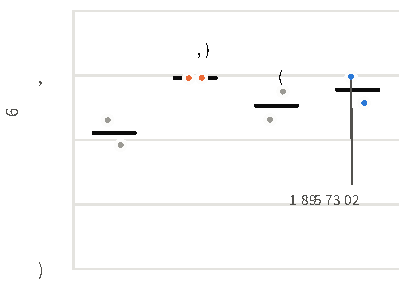
\includegraphics[width=\linewidth]{scarcity-ko.pdf}
    \caption{E1: 저메모리 전경 작업의 완료 시간. 점은 블록별 값, 가로선은 중앙값이다. 실제 축소가 일어난 반복(왼쪽 파란 점)이 가장 느렸다.}
    \label{fig:scarcity}
  \end{minipage}\hfill
  \begin{minipage}[b]{0.49\linewidth}
    \centering
    \small
    \begin{tabular}{@{}lrr@{}}
      \toprule
      조건 & 중앙값 (ms) & 축소 \\
      \midrule
      여유 RAM (참고) & \numScAmb & 0 \\
      저메모리 · 미실행 & \numScAbs & 0 \\
      저메모리 · 관찰만 & \numScDry & 0 \\
      저메모리 · 실제 관리 & \numScLive & 1 \\
      \midrule
      실제 관리 $-$ 미실행 & \multicolumn{2}{l}{\numScDiff\ ms (\numScDiffPct\%)} \\
      \bottomrule
    \end{tabular}
    \captionof{table}{E1 요약(조건당 2회). 음수는 더 빨랐다는 뜻이다.}
    \label{tab:scarcity}
  \end{minipage}
\end{figure}

이보다 앞서 가용 RAM이 약 2.5\,GiB 남은 상태에서 수행한 비교에서는, 배경 앱의 상주량이 중앙값 약 1,055.6\,MiB 줄었지만 시스템 가용 RAM은 약 13.3\,MiB만 늘었고, 그 배경 앱을 다시 쓸 때의 재접근 시간은 54.5\,ms에서 240.5\,ms로 길어졌다. 상주량 감소, 사용 가능 메모리 증가, 응답성 개선은 서로 다른 지표라는 점\citep{mswset,russinovich2004}이 그대로 드러난 것이다. 이 결과로 ``가용 물리 RAM이 1\,GiB 이상이면 강제 축소를 보류한다''는 규칙을 추가했다. 비활성 시계만 가속한 회귀 재현에서 수정 후 재접근 시간 중앙값은 238.36\,ms에서 56.94\,ms가 되었다. 이것은 불필요한 회수의 비용을 막았다는 근거이지, 저메모리 성능 향상의 근거는 아니다.

\finding{\textbf{RQ1 답.} Working Set 축소는 사용 가능 메모리 숫자를 키울 수 있지만, 이 실험들에서는 전경 작업을 빠르게 하지 못했고 여유가 있을 때는 복귀를 느리게 했다. 그래서 설계의 중심을 ``메모리 비우기''에서 ``배경 작업의 명시적 양보''로 옮겼다.}

\subsection{RQ2: 명시적 배경 양보는 통제 부하에서 p95를 크게 줄였다}
\label{sec:rq2}

\begin{figure}[t]
  \centering
  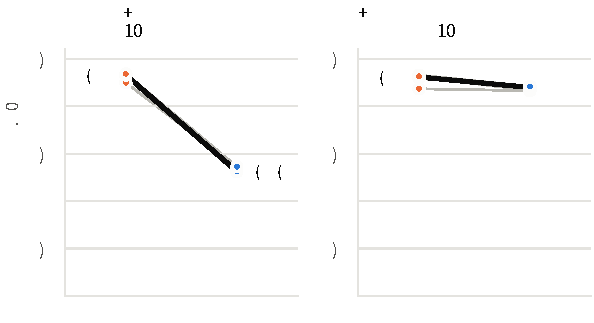
\includegraphics[width=0.66\linewidth]{background-control-ko.pdf}
  \caption{E2: 블록별 전경 요청 p95. 메모리+CPU 경쟁에서는 다섯 블록 모두 크게 줄었지만, CPU 경쟁만 있을 때(이전 엔진은 조정 0회)는 차이가 작았다.}
  \label{fig:bgc}
\end{figure}

\begin{table}[t]
\centering\small
\begin{tabular}{@{}lrrrrrr@{}}
\toprule
& \multicolumn{2}{c}{p50 중앙값 (ms)} & \multicolumn{2}{c}{p95 중앙값 (ms)} & p95 감소 & 배경 처리량 \\
\cmidrule(lr){2-3}\cmidrule(lr){4-5}
비교 & 기준 & 수정 & 기준 & 수정 & {\scriptsize [블록 범위]} & 감소 \\
\midrule
메모리+CPU (미실행 vs 수정) & \numMxOffFifty & \numMxOnFifty & \numMxOff & \numMxOn & \numMxRed\% {\scriptsize[\numMxBlkMin, \numMxBlkMax]} & \numMxBgRed\% \\
CPU만 (이전 vs 수정) & \numCpOffFifty & \numCpOnFifty & \numCpOff & \numCpOn & \numCpRed\% {\scriptsize[\numCpBlkMin, \numCpBlkMax]} & \numCpBgRed\% \\
\bottomrule
\end{tabular}
\caption{E2 결과(각 5블록, 블록당 조건별 60요청). 두 비교 모두 5/5 블록에서 p95가 줄었다.}
\label{tab:bgc}
\end{table}

표~\ref{tab:bgc}와 그림~\ref{fig:bgc}에서 메모리+CPU 경쟁의 p95 중앙값은 \numMxOff\,ms에서 \numMxOn\,ms로 \numMxRed\% 줄었다. 블록별 감소는 \numMxBlkMin--\numMxBlkMax\% 로 좁은 범위에 모였고, 기하평균 감소의 95\% 신뢰구간은 [\numMxGmLo, \numMxGmHi]\%였다. 수정 조건에서는 매번 배경 프로세스 8개에 실제 조정이 적용되었다. 작업 직전 가용 RAM은 \numMxAvLo--\numMxAvHi\,MiB였다.

흥미로운 것은 CPU 경쟁만 있는 비교이다. 중간값(p50)은 \numCpOffFifty\,ms에서 \numCpOnFifty\,ms로 \numCpFiftyRed\% 줄었지만, p95는 \numCpRed\% 줄어드는 데 그쳤다. 즉 대부분의 요청은 빨라졌어도 가장 느린 요청들은 여전히 느렸다. 평균이나 중앙값만 보고하면 효과를 과대평가할 수 있다는 뜻이며\citep{dean2013tail}, 이 결과도 제외하지 않고 보고한다. 메모리 압박이 함께 있을 때 꼬리까지 줄어든 원인이 메모리 우선순위인지, CPU 우선순위·EcoQoS와의 결합인지는 이 설계로 분리할 수 없다(\S\ref{sec:threats}).

\finding{\textbf{RQ2 답.} 메모리와 CPU가 함께 부족한 통제 부하에서, 지정한 배경 작업을 양보시키자 전경 p95가 5/5 블록에서 약 40--44\% 줄었다. CPU 경쟁만 있을 때는 중간값은 줄었지만 꼬리는 거의 줄지 않았다.}

\subsection{RQ3: 효과는 실제 Chrome과 VS Code로 옮겨 갔다}
\label{sec:rq3}

\begin{figure}[t]
  \centering
  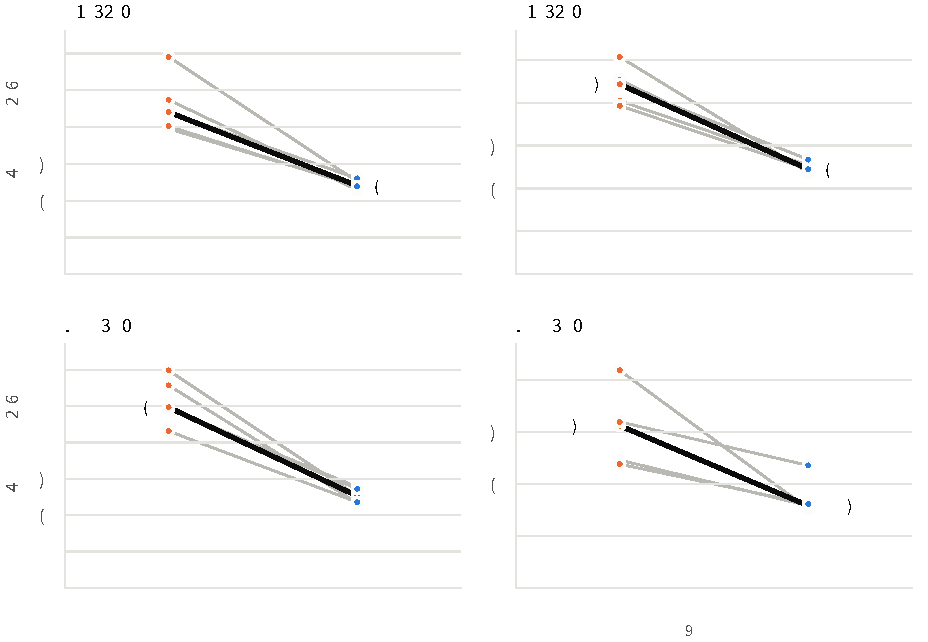
\includegraphics[width=0.92\linewidth]{real-apps-ko.pdf}
  \caption{E3: 실제 앱 기능의 블록별 p95. 네 기능 모두 다섯 쌍 전부에서 지연이 줄었다.}
  \label{fig:real}
\end{figure}

\begin{table}[t]
\centering\small
\setlength{\tabcolsep}{4.5pt}
\begin{tabular}{@{}lrrrrrc@{}}
\toprule
& \multicolumn{2}{c}{p95 중앙값 (ms)} & & & 기하평균 감소 & 개선 \\
\cmidrule(lr){2-3}
기능 & 미사용 & 사용 & 감소 & 블록 범위 & 95\% 신뢰구간 & 블록 \\
\midrule
Chrome 검색 $\rightarrow$ 렌더링 경계 & \numCSOff & \numCSOn & \numCSRed\% & \numCSBlkMin--\numCSBlkMax\% & [\numCSGmLo, \numCSGmHi]\% & 5/5 \\
Chrome 정렬 $\rightarrow$ 렌더링 경계 & \numCOOff & \numCOOn & \numCORed\% & \numCOBlkMin--\numCOBlkMax\% & [\numCOGmLo, \numCOGmHi]\% & 5/5 \\
VS Code 편집 $\rightarrow$ 코드 완성 & \numVCOff & \numVCOn & \numVCRed\% & \numVCBlkMin--\numVCBlkMax\% & [\numVCGmLo, \numVCGmHi]\% & 5/5 \\
VS Code 편집 $\rightarrow$ 저장 & \numVSOff & \numVSOn & \numVSRed\% & \numVSBlkMin--\numVSBlkMax\% & [\numVSGmLo, \numVSGmHi]\% & 5/5 \\
\bottomrule
\end{tabular}
\caption{E3 결과. 각 값은 세션별 30회 작업의 p95를 먼저 구한 뒤 5개 블록의 중앙값을 계산한 것이다. 기능별 정확 부호검정 단측 $p=\numSignP$.}
\label{tab:real}
\end{table}

표~\ref{tab:real}과 그림~\ref{fig:real}에서 네 기능의 p95 지연은 \numCSRed--\numVSRed\% 줄었다. 다섯 블록 모두에서 개선되었으므로 기능별 정확 부호검정의 단측 $p$는 \numSignP 이다. 블록 수가 5개라 양측 Wilcoxon 검정은 가능한 최솟값인 $p=\numWilP$ 에 머문다. 기능들이 같은 세션을 공유하므로, 독립 단위인 \emph{앱 세션}으로 묶어 보면 \numSessions{}개 세션 모두에서 그 세션의 모든 기능이 개선되었고 양측 부호검정 $p=\numPooledP$ 이다.

Chrome 값에는 자동화 통신의 왕복이 포함된다. 페이지 안에서 잰 입력 이벤트부터 두 번째 rAF 경계까지의 p95 중앙값도 검색 \numEfSOff$\rightarrow$\numEfSOn\,ms, 정렬 \numEfOOff$\rightarrow$\numEfOOn\,ms로 같은 방향이었다. 미사용 조건의 지연(62--99\,ms)은 사람이 ``즉각적''이라고 느끼는 0.1초 경계\citep{card1991} 근처이고, 사용 조건(32--51\,ms)은 그보다 확실히 아래이다. 다만 두 번째 rAF는 렌더링 기회의 경계일 뿐 화면 표시 완료를 보장하지 않고, VS Code 값은 API 완료 시간이지 키 입력부터 추천 창이 보일 때까지의 시간이 아니다.

\finding{\textbf{RQ3 답.} 통제 부하에서 본 효과는 실제 브라우저 렌더러와 편집기 기능으로 옮겨 갔다. 네 기능 모두 5/5 블록에서 p95가 약 45--49\% 줄었다.}

\subsection{RQ4: 대가는 배경 처리량이며, 조정은 안전하게 원복되었다}
\label{sec:rq4}

\begin{figure}[t]
  \centering
  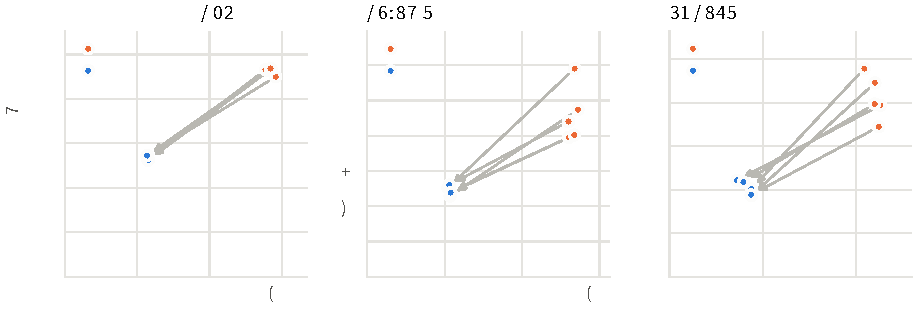
\includegraphics[width=\linewidth]{tradeoff-ko.pdf}
  \caption{전경 응답과 배경 처리량의 교환. 각 화살표는 한 블록이 미사용(주황)에서 사용(파랑)으로 이동한 것이다. 모든 점이 왼쪽 아래로 움직였다: 전경은 빨라지고 배경은 느려진다.}
  \label{fig:tradeoff}
\end{figure}

그림~\ref{fig:tradeoff}는 이 연구의 핵심 결과를 한 장으로 보여준다. 배경 처리량(초당 처리한 64\,KiB 조각 수)은 E2에서 \numMxBgRed\%, E3의 Chrome에서 \numBgCRed\%(\numBgCOff$\rightarrow$\numBgCOn), VS Code에서 \numBgVRed\%(\numBgVOff$\rightarrow$\numBgVOn) 줄었다. RamFlow는 총 처리량을 늘린 것이 아니라 \emph{누가 먼저 자원을 쓰는지}를 바꾸었다. 이 값은 전경 작업 구간 동안의 진행 속도이므로, 배경 작업의 전체 완료 시간이 같은 비율로 늘어난다고 해석해서는 안 된다. ProBalance 문서는 우선순위를 낮춰도 배경 작업이 거의 같은 시간에 끝난다고 설명하는데\citep{probalance}, 우리 부하처럼 CPU와 메모리를 계속 다투는 경우에는 배경 진행이 크게 느려질 수 있음을 보여준다. 그래서 RamFlow는 기본 보호를 일괄 해제하지 않고, 사용자가 \emph{양보해도 되는} 작업을 실행 파일 경로로 지정하게 했다.

\paragraph{안전성과 정확성}
E2와 E3의 본 실험 40개 조건, 총 2,400개의 전경 요청·기능 작업에서 다음을 확인했다. 대상 밖 변경 요청 0회, 안전 부하 해제 0회, 모든 조건에서 우선순위·전력·CPU Sets 값이 처음 값으로 원복, E2의 1,200개 요청 결과 해시 일치, E3의 모든 검색·정렬 결과 및 코드 완성 필드 검증 통과, VS Code 대응 쌍별 최종 저장 해시 일치, 측정 전후 앱 실행 파일 해시 일치. 측정에 쓴 Core의 SHA-256은 E2·E3 모두 \code{d64160b8\ldots8b93}으로 같았고, 이번 검증을 위해 정책이나 실행 파일을 바꾸지 않았다. 자동 회귀 검사로는 Windows API·IPC·실제 큐 자식 실행을 포함한 218개 assertion, 저장소 26개, 외부 관찰기 38개, 기존 Python 70개가 통과했다.

\finding{\textbf{RQ4 답.} 전경 p95 약 45\% 감소의 대가는 지정한 배경 작업 처리량 약 60\% 감소였다. 조정은 매번 처음 값으로 원복되었고 대상 밖 변경은 없었다.}

%=====================================================================
\section{논의}
\label{sec:discussion}

\paragraph{``가용 RAM''은 목표가 아니라 지표이다}
E1과 앞선 비교는 RAM 최적화기에 대한 오래된 비판\citep{russinovich2004}을 현대 Windows 11에서 다시 확인한다. 사용 가능 메모리 숫자는 쉽게 키울 수 있지만, 사용자가 원하는 것은 지금 쓰는 앱의 빠른 응답이다. 측정해야 할 것은 전경 작업의 지연이며, 숫자를 키우는 조치는 그 비용(재접근 지연)까지 함께 재야 한다.

\paragraph{누구를 기다리게 할 것인가}
자원이 부족할 때 할 수 있는 일은 결국 순서를 정하는 것이다. RamFlow의 결과는 ``사용자가 기다려도 된다고 표시한 작업''을 뒤로 미루면 전경 꼬리 지연이 크게 줄어든다는 것을 보여준다. 이 결정을 자동으로 추측하면 중요한 배경 작업(녹화, 내려받기, 빌드)을 해칠 수 있으므로, 자동 관리는 30분 비활성·활동 확인 등으로 보수적으로 두고 공격적인 양보는 사용자의 명시적 지정에만 허용했다.

\paragraph{중앙값과 꼬리는 다르게 움직인다}
CPU 경쟁만 있는 비교에서 p50은 43\% 줄었지만 p95는 4.8\% 줄었다. 응답성 도구를 평가할 때 평균이나 중앙값만 보고하면 체감 효과를 과장할 수 있다. 우리는 꼬리를 주 지표로 정하고, 불리한 결과도 함께 공개했다.

\paragraph{다른 운영체제로의 이식}
리눅스에서는 PSI가 ``멈춘 시간''을 직접 제공하고\citep{psi}, cgroup v2가 메모리·CPU 가중치를 프로세스 묶음 단위로 조정할 수 있어, 같은 정책을 더 정확한 신호로 구현할 여지가 있다\citep{weiner2022tmo}. RamFlow의 리눅스판은 별도 저장소에서 개발 중이며, 이 논문의 측정 범위에는 포함하지 않는다.

%=====================================================================
\section{타당성 위협}
\label{sec:threats}

\paragraph{외적 타당성}
모든 측정은 한 대의 PC(24\,GiB, 하이브리드 CPU)에서 이루어졌다. 8\,GiB PC, 다른 CPU, 노트북 배터리 상태에서는 결과가 다를 수 있다. 배경 부하는 실제 빌드·내려받기·AI 추론이 아닌 합성 SHA-256 작업이다. E3에서 전경은 실제 앱이지만, 일반 웹사이트나 개인 프로젝트가 아닌 생성된 로컬 페이지와 문서를 썼다.

\paragraph{구성 타당성}
Chrome 지표는 자동화 왕복을 포함하고 화면 표시 완료를 보장하지 않으며, VS Code 지표는 API 완료 시간이다. 물리 키 입력 지연, 프레임 지연, 게임 FPS는 재지 않았다. 배경 처리량은 전경 작업 구간의 진행 속도이다.

\paragraph{내적 타당성}
E2·E3의 사용 조건은 메모리 우선순위·CPU 우선순위·EcoQoS를 함께 바꾸었으므로 각 요소의 기여를 분리할 수 없다. 사용 조건에는 엔진과 트레이가 실제로 실행되어 그 메모리 비용이 포함되지만, 엔진은 측정용 테스트 호스트에서 실행되었다(센서·정책·설정 함수·원복은 실제 동작). 외부 메모리 할당량을 조건별로 다시 맞추지 않았기 때문에, Windows의 자연 회수에 따라 작업 직전 가용 RAM이 블록마다 달랐다(값은 CSV에 기록). E1은 블록 2개뿐이고 압박 수준도 같지 않았다.

\paragraph{통계적 결론 타당성}
각 비교의 블록 수는 5개이다. 5/5 개선이라는 일관성은 강하지만, 양측 정확 검정의 최소 $p$가 0.0625이므로 기능별로는 통상의 0.05 기준을 양측에서 넘을 수 없다. 앱 세션 단위의 통합 부호검정($p=\numPooledP$)은 기능 간 상관을 피하기 위한 보수적 묶음이다. 여러 기능을 검정했으나 다중 비교 보정은 하지 않았다. 효과 크기가 크고 방향이 일관되어 결론이 바뀌지는 않지만, 더 많은 PC와 블록으로 재현하는 것이 필요하다\citep{kalibera2013}.

%=====================================================================
\section{결론}
\label{sec:conclusion}

RamFlow는 ``RAM을 최대한 비운다''는 목표를 버리고 ``현재 작업을 보호하면서 압박에 보수적으로 대응한다''는 목표로 설계한 Windows 자원 조정 도구이다. 실측 결과, Working Set 축소 위주의 정책은 전경 이득을 보이지 못했고, 사용자가 지정한 배경 작업에 되돌릴 수 있는 양보를 요구하는 정책은 통제 부하와 실제 Chrome·VS Code에서 p95 지연을 약 44--49\% 줄였다. 그 대가는 배경 처리량 약 60\% 감소였다. 앞으로는 (i) 메모리 우선순위·CPU 우선순위·EcoQoS의 개별 기여 분리, (ii) 양보 정도를 연속적으로 조절하는 정책, (iii) 빠른 앱 전환과 8\,GiB급 PC를 포함한 다기종 재현, (iv) PSI를 쓰는 리눅스판과의 비교를 진행할 계획이다.

{\small
\renewcommand{\refname}{참고문헌}
\begin{thebibliography}{99}

\bibitem{denning1968}
P.~J. Denning.
\newblock The working set model for program behavior.
\newblock \emph{Communications of the ACM}, 11(5):323--333, 1968.

\bibitem{mswset}
Microsoft.
\newblock Working set.
\newblock Win32 documentation, \url{https://learn.microsoft.com/en-us/windows/win32/memory/working-set}.

\bibitem{russinovich2004}
M.~Russinovich.
\newblock The memory-optimization hoax: {RAM} optimizers make false promises.
\newblock \emph{Windows IT Pro}, Jan.\ 2004.
\newblock \url{https://www.itprotoday.com/cloud-computing/memory-optimization-hoax}.

\bibitem{chen2021softram}
R.~Chen.
\newblock Analysis of {SoftRAM 95}.
\newblock \emph{The Old New Thing}, Microsoft DevBlogs, Nov.\ 2021.
\newblock \url{https://devblogs.microsoft.com/oldnewthing/20211111-00/?p=105897}.

\bibitem{win10compression}
Microsoft Windows Insider Program.
\newblock Windows 10: Memory compression.
\newblock Windows Insider Hub, Aug.\ 2015 (build 10525).

\bibitem{mavericks2013}
Apple Inc.
\newblock {OS X Mavericks}: Core technologies overview (Compressed Memory, App Nap).
\newblock Technology overview, 2013.

\bibitem{powerthrottling2017}
B.~Karagounis.
\newblock Introducing power throttling.
\newblock Windows Blogs, Apr.\ 2017.
\newblock \url{https://blogs.windows.com/windowsexperience/2017/04/18/introducing-power-throttling/}.

\bibitem{ecoqos2021}
R.~Li.
\newblock Introducing {EcoQoS}.
\newblock Microsoft DevBlogs (Sustainable Software), 2021.
\newblock \url{https://devblogs.microsoft.com/sustainable-software/introducing-ecoqos/}.

\bibitem{mssetprocinfo}
Microsoft.
\newblock {SetProcessInformation} function (processthreadsapi.h).
\newblock Win32 documentation, \url{https://learn.microsoft.com/windows/win32/api/processthreadsapi/nf-processthreadsapi-setprocessinformation}.

\bibitem{mscpusets}
Microsoft.
\newblock {CPU} sets.
\newblock Win32 documentation, \url{https://learn.microsoft.com/windows/win32/procthread/cpu-sets}.

\bibitem{mspriority}
Microsoft.
\newblock {SetPriorityClass} function (processthreadsapi.h).
\newblock Win32 documentation, \url{https://learn.microsoft.com/windows/win32/api/processthreadsapi/nf-processthreadsapi-setpriorityclass}.

\bibitem{mspipe}
Microsoft.
\newblock Named pipe security and access rights.
\newblock Win32 documentation, \url{https://learn.microsoft.com/windows/win32/ipc/named-pipe-security-and-access-rights}.

\bibitem{probalance}
Bitsum.
\newblock {ProBalance} --- Process Lasso documentation.
\newblock \url{https://bitsum.com/apps/process-lasso/docs/algorithms/probalance/}.

\bibitem{weiner2022tmo}
J.~Weiner, N.~Agarwal, D.~Schatzberg, L.~Yang, H.~Wang, B.~Sanouillet, B.~Sharma, T.~Heo, M.~Jain, C.~Tang, and D.~Skarlatos.
\newblock {TMO}: Transparent memory offloading in datacenters.
\newblock In \emph{Proc.\ ASPLOS '22}, 2022.
\newblock \url{https://doi.org/10.1145/3503222.3507731}.

\bibitem{psi}
The Linux kernel documentation.
\newblock {PSI} --- Pressure stall information.
\newblock \url{https://docs.kernel.org/accounting/psi.html}.

\bibitem{lmkd}
Android Open Source Project.
\newblock Low memory killer daemon.
\newblock \url{https://source.android.com/docs/core/perf/lmkd}.

\bibitem{dean2013tail}
J.~Dean and L.~A. Barroso.
\newblock The tail at scale.
\newblock \emph{Communications of the ACM}, 56(2):74--80, 2013.

\bibitem{card1991}
S.~K. Card, G.~G. Robertson, and J.~D. Mackinlay.
\newblock The information visualizer, an information workspace.
\newblock In \emph{Proc.\ CHI '91}, pages 181--186, 1991.

\bibitem{mytkowicz2009}
T.~Mytkowicz, A.~Diwan, M.~Hauswirth, and P.~F. Sweeney.
\newblock Producing wrong data without doing anything obviously wrong!
\newblock In \emph{Proc.\ ASPLOS XIV}, pages 265--276, 2009.

\bibitem{kalibera2013}
T.~Kalibera and R.~Jones.
\newblock Rigorous benchmarking in reasonable time.
\newblock In \emph{Proc.\ ISMM '13}, pages 63--74, 2013.

\bibitem{jain1991}
R.~Jain.
\newblock \emph{The Art of Computer Systems Performance Analysis}.
\newblock Wiley, 1991.

\bibitem{cdp}
Chrome for Developers.
\newblock Changes to remote debugging switches to improve security.
\newblock \url{https://developer.chrome.com/blog/remote-debugging-port}.

\bibitem{vscodetest}
Visual Studio Code.
\newblock Testing extensions; Built-in commands.
\newblock \url{https://code.visualstudio.com/api/working-with-extensions/testing-extension}.

\end{thebibliography}

}

\appendix
\section{재현 방법}
\label{app:repro}
저장소의 \code{docs/evidence/}에 조건별 요약 CSV와 프로토콜·해시 JSON이 있다. 이 논문의 모든 수치(\code{paper/shared/numbers.tex})와 그림(\code{paper/figures/})은 다음 명령으로 다시 만들 수 있다.
\begin{center}
\small\code{python3 paper/analysis/analyze.py}\qquad\code{cd paper/ko \&\& xelatex main \&\& xelatex main}
\end{center}
분석에는 Python 3, numpy, scipy, matplotlib가 필요하고, 조판에는 XeLaTeX, \code{xetexko}, Noto CJK 글꼴이 필요하다. 측정 원본(요청별 기록, 원시 센서, 이벤트, 실행 소스)은 용량 때문에 Git에서 제외하고 로컬 \code{benchmarks/}에 보존했으며, 요약 CSV가 본문 분석의 입력이다. 제품 빌드와 회귀 검사는 저장소의 \code{README.ko.md}에 있다.

\begin{table}[h]
\centering\small
\begin{tabularx}{\linewidth}{@{}lX@{}}
\toprule
자료 & 위치 \\
\midrule
E1 저메모리 & \code{docs/evidence/2026-11-09-scarcity/\{trials.csv, summary.json\}} \\
E2 배경 제어 & \code{docs/evidence/2026-11-09-background-control/\{trials.csv, summary.json\}} \\
E3 실제 앱 & \code{docs/evidence/2026-11-10-real-apps/\{trials.csv, summary.json\}} \\
분석 결과 & \code{paper/analysis/stats.json} \\
정책 코드 & \code{native/RamFlow.Core/Policy.cs}, \code{Engine.cs}, \code{BackgroundJobs.cs} \\
\bottomrule
\end{tabularx}
\end{table}

\end{document}
